\section{BDD radon}

\subsection{Importation}

\subsubsection{Transformation du fichier xlsx en csv}
A partir du fichier source au format \textit{xlsx}, nous utilisons le programme Excel 2016 pour exporter les données dans un format plus facile à traiter par OpenRefine. Lorsque le fichier est ouvert avec Excel 2016, il faut suivre les étapes suivantes: Fichier $>$ Exporter $>$ Modifier le type de fichier $>$ CSV (séparateur: point-virgule) (*.csv) $>$ Enregistrer sous.

\subsubsection{Nettoyage par OpenRefine}
Nous devons à présent passer le fichier par OpenRefine afin d'éliminer des colonnes inutiles et de transformer les données dans un format acceptable par notre programme. Pour ce faire, il faut créer un nouveau projet OpenRefine à partir du fichier csv crée précedemment, puis l'exporter en appliquant les options d'exportation trouvable dans la source du programme sous "metadata/rn-db\_openrefine-options.json". Une chose à ne pas oublier lors de cette étape est de cocher la case "Ignore facets and filters and export all rows" afin d'exporter toutes les lignes du fichier.

Le fichier ainsi généré doit être placé sous "data/rn-db/main.csv"

\subsection{Prétraitement}

La BDD radon ne nécessite pas de prétraitement avant de pouvoir être utilisée par le programme. Il faut cependant que les dates de début et de fin de la mesure du radon (colonnes START\_TIME et END\_TIME) soient transformées au format ISO 8601. La transformation de la date est faite par Spark en lui fournissant comme option d'importation "dateFormat" $\rightarrow$ "dd.MM.yyyy". 

Pour connaître les champs de la BDD qui sont utilisés dans le programme, voir "src/main/scala/data/RadonDatabase.scala" (voir annexe \ref{sectionRadonDatabaseScala}). 

\section{Étage moyen d'habitation}

\subsection{Importation}
Nous transformons le fichier téléchargé à la section \ref{sectionCantonEtagesBatiments} à l'aide d'OpenRefine. Les options par défault peuvent être gardées pour créer le projet OpenRefine. Il faut ensuite utiliser les options d'exportation trouvables dans le fichier suivant: "metadata/canton-floors-buildings\_openrefine-options.json" pour exporter le fichier traité.

Le fichier ainsi généré doit être placé sous "data/avg-floor/2020/main.csv"

\subsection{Prétraitement}

Pour plus de détails sur les opérations décrites dans cette section, veuillez vous référer à "src/main/scala/data/AverageFloor2020.scala" (voir annexe \ref{sectionAverageFloor2020Scala}). 
\subsubsection{Conversion des colonnes en format utile}
Les colonnes "Canton" et "Nombre d'étages" doivent être traitées avant de pouvoir être utilisées car elles ont un format non compatible avec les autres sources de données. 
\begin{itemize}
\item Pour la colonne "Canton", chaque nom de canton écrit en toutes lettres est converti dans le code à 2 lettres du canton (exemple "Bern / Berne" $\rightarrow$ "BE")
\item Pour la colonne "Nombre d'étages", chaque description du nombre d'étages est converti en un nombre simple (exemple "4 ét." $\rightarrow$ 4, "10+ ét." $\rightarrow$ 10\footnote{On notera d'ailleurs ici qu'une partie du sens des données initiales est perdu comme on considère que tous les bâtiments qui ont \textbf{plus de} 10 étages ont \textbf{exactement} 10 étages. Cette simplification ne devrait cependant pas avoir un impact significatif sur le résultat comme la majorité des bâtiments en Suisse ont moins de 10 étages (ceci est visible facilement dans les données du nombre d'étage des bâtiments par canton).})
\end{itemize}

\subsubsection{Calcul de l'étage d'habitation moyen par canton}\label{importationEtageMoyen}
Pour calculer l'étage moyen d'habitation par canton, nous utilisons la moyenne pondérée du nombre d'étages par le nombre de bâtiments qui ont ce nombre d'étages:

\begin{equation}
E_c = \frac{1}{2} \cdot \frac{\sum_{e=1}^{10} n_{e,c} \cdot e}{\sum_{e=1}^{10} n_{e,c}}
\end{equation}

où

\begin{itemize}
\item $E_c$ représente l'étage moyen d'habitation dans le canton $c$
\item $n_{e,c}$ représente le nombre de bâtiments qui ont $e$ étages dans le canton $c$
\end{itemize}

Il est très important de noter ici qu'il faut distinguer le \textbf{nombre} d'étages, et l'étage moyen \textbf{d'habitation}. C'est pour cette raison que nous multiplions la moyenne pondérée du \textbf{nombre} d'étages par un facteur $\frac{1}{2}$. Nous pouvons en effet observer que par exemple, pour un bâtiment de 5 étages, les habitants résident en moyenne à l'étage 2.5 (en supposant que tous les étages sont uniformément occupés).

Ci-dessous, nous montrons les valeurs de l'étage moyen d'habitation par canton, en 2004, 2009 et 2020. Les données de 2004 sont issues du document cité à la section \ref{sectionReferenceCalcul}. Les données pour 2009 et 2020 sont calculées à partir du nombre d'étages par bâtiment (données de l'OFS). Les valeurs pour 2004 et 2009 sont données comme points de comparaison avec les valeurs de 2020 qui sont utilisées pour le calcul de la valeur moyenne de la concentration de radon. 
Il est important de noter ici, que les différences entre les valeurs de 2004 et 2009 sont plus importantes qu'entre 2009 et 2020. Un exemple frappant est la valeur pour le canton de Genève qui passe de 2.89 en 2004 à 1.67 en 2009 et reste à 1.67 en 2020. Ceci nous laisse à penser qu'il y a une différence dans la méthode de calcul ou dans la source des données entre ce qui avait été calculé en 2004 et ce que nous avons calculé pour 2009 et 2020. Cependant il nous est impossible d'être certain d'où vient la différence car le rapport de 2004 est imprécis sur la source de ces données. La seule indication qui nous est donnée est: "Quelle: Bundesamt für Statistik" (en français: "Source: Office fédéral de la statistique"). 
Nous considérons cependant que notre source de données et notre méthode de calcul semblent correctes et nous utiliserons donc les valeurs d'étage moyen d'habitation pour 2020 que nous avons calculées pour la suite des calculs.
\pagebreak

\begin{center}
\begin{multicols}{3}[Étage moyen d'habitation, en 2004, en 2009 et en 2020 respectivement]
\csvautotabular{../data/avg-floor/2004/avg-floor-per-canton-2004-COMMA_CSV.csv}
\csvautotabular{../data/avg-floor/2009/computed-avg/kanton-etage.csv}
\csvautotabular{../data/avg-floor/2020/computed-avg/kanton-etage.csv}
\end{multicols}
\end{center}

\section{Nombre d'habitants par commune}
\subsection{Importation}

À partir du fichier \textit{xlsx} téléchargé à la section \ref{sectionNombreHabitantsCommunes}, nous utilisons OpenRefine pour transformer les données dans un format traitable par notre programme.

Les options d'importation pour OpenRefine doivent être ajustées pour traiter correctement le fichier \textit{xlsx} qui a une structure peu régulière. Veuillez vous référer à la figure \ref{fig:importPopulationPerTownOpenRefine}.

\begin{figure}[H]
    \centering
    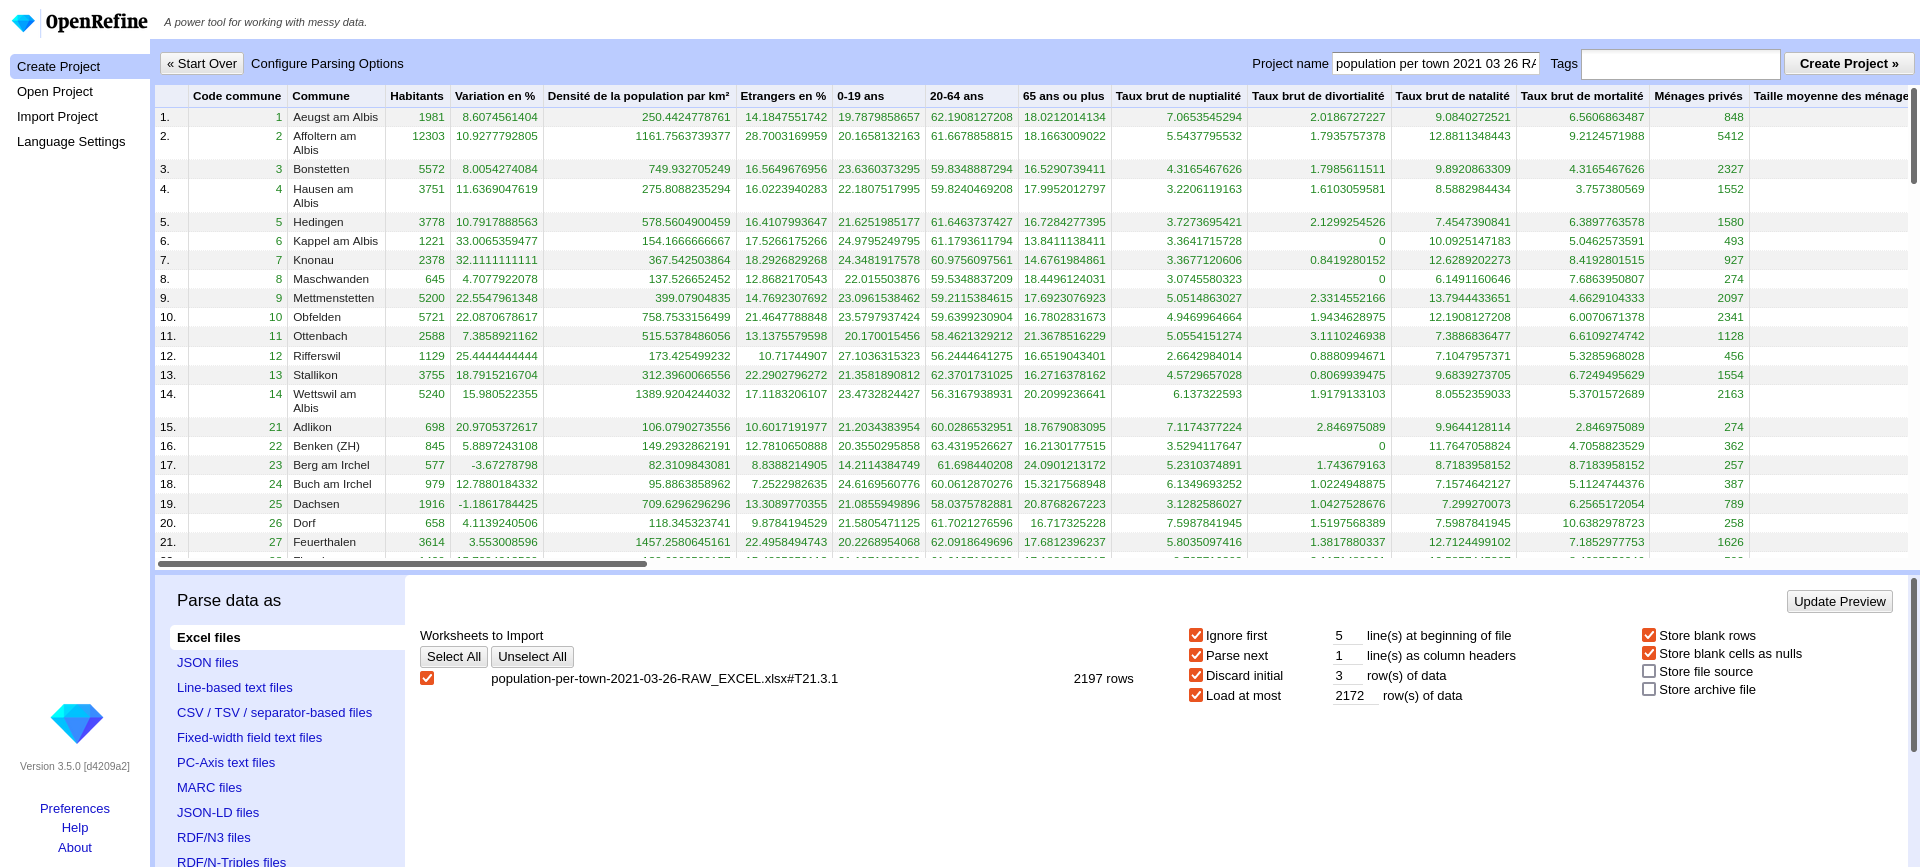
\includegraphics[width=\textwidth]{import-population-per-town-OPENREFINE}
    \caption{Options à sélectionner pour créer le projet OpenRefine. Ignore first = 5, Parse next = 1, Discard initial = 3, Load at most = 2172}
    \label{fig:importPopulationPerTownOpenRefine}
\end{figure}

Il faut ensuite utiliser les options d'exportation trouvables dans le fichier suivant: "metadata/population-per-town\_openrefine-options.json" pour exporter le fichier traité.

Le fichier ainsi généré doit être placé sous "data/population-per-town/main.csv".

\subsection{Prétraitement}
Le seul prétraitement qui doit être effectué est de convertir les nombres (numéro de commune et population correspondante) d'un type de nombre réel (avec des $.0$ en suffixe) en nombre entier. Ceci est fait dans "src/main/scala/data/TownPopulations.scala".